% Diagrama B — estrutura informacional ilustrativa entre canais e alvo.
% Não representa um grafo causal.
\documentclass[tikz,border=6pt]{standalone}
% Preâmbulo compartilhado dos diagramas conceituais do relatório CoInfoSim.
% Compilação: xelatex (determinística; nenhum dado experimental é usado).
\usepackage{fontspec}
\setmainfont{Liberation Sans}
\setsansfont{Liberation Sans}
\usepackage{amsmath}
\usepackage{bm}
\usepackage{tikz}
\usetikzlibrary{arrows.meta,positioning,calc,fit,backgrounds,decorations.pathreplacing,matrix,patterns}
\definecolor{CoinAccent}{RGB}{25,80,140}
\definecolor{CoinAccentDark}{RGB}{18,55,95}
\definecolor{CoinAccentPale}{RGB}{237,242,248}
\definecolor{CoinGray}{RGB}{95,95,95}
\definecolor{CoinGrayPale}{RGB}{246,246,246}
\definecolor{CoinWin}{RGB}{76,140,90}    % verde discreto (vitória)
\definecolor{CoinLose}{RGB}{182,88,79}   % vermelho discreto (derrota)
\tikzset{
  bloco/.style={draw=CoinAccentDark, fill=CoinAccentPale, rounded corners=1.2pt,
                align=center, font=\small, inner sep=4pt, minimum height=7mm},
  bloconeutro/.style={draw=CoinGray, fill=CoinGrayPale, rounded corners=1.2pt,
                align=center, font=\small, inner sep=4pt, minimum height=7mm},
  blocoreal/.style={draw=CoinAccentDark, fill=white, rounded corners=1.2pt,
                align=center, font=\small, inner sep=4pt, minimum height=7mm},
  seta/.style={-{Stealth[length=2.4mm]}, thick, CoinAccentDark},
  setacinza/.style={-{Stealth[length=2.4mm]}, thick, CoinGray},
  rotulo/.style={font=\footnotesize\itshape, text=CoinGray, align=center},
}

\begin{document}
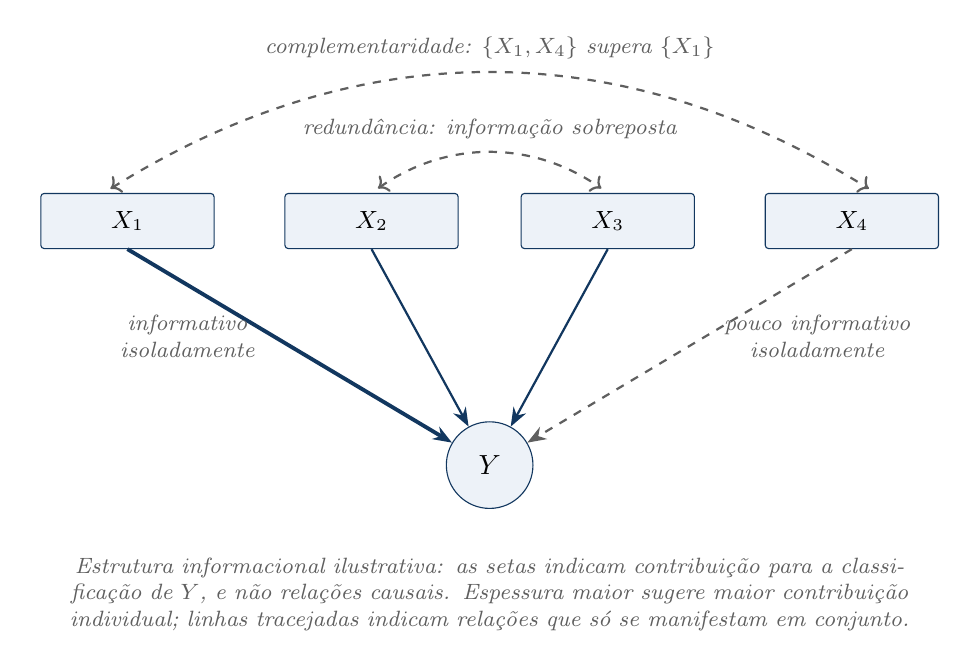
\begin{tikzpicture}
  % Alvo
  \node[circle, draw=CoinAccentDark, fill=CoinAccentPale, font=\bfseries, minimum size=11mm] (Y) at (0,0) {$Y$};

  % Canais
  \node[bloco, minimum width=2.2cm] (X1) at (-4.6,3.1) {$X_1$};
  \node[bloco, minimum width=2.2cm] (X2) at (-1.5,3.1) {$X_2$};
  \node[bloco, minimum width=2.2cm] (X3) at (1.5,3.1)  {$X_3$};
  \node[bloco, minimum width=2.2cm] (X4) at (4.6,3.1)  {$X_4$};

  % X1: forte isolado
  \draw[seta, line width=1.4pt] (X1.south) -- (Y)
    node[pos=0.45, left=1mm, rotulo] {informativo\\isoladamente};
  % X2 e X3: individualmente úteis, mas redundantes entre si
  \draw[seta] (X2.south) -- (Y);
  \draw[seta] (X3.south) -- (Y);
  \draw[setacinza, dashed, <->, shorten >=1mm, shorten <=1mm] (X2.north) to[bend left=35]
    node[above=0.5mm, rotulo] {redundância: informação sobreposta} (X3.north);
  % X4: fraco isolado, útil em combinação com X1
  \draw[setacinza, dashed] (X4.south) -- (Y)
    node[pos=0.45, right=1mm, rotulo] {pouco informativo\\isoladamente};
  \draw[setacinza, dashed, <->, shorten >=1mm, shorten <=1mm]
    ($(X1.north)+(-0.3,0)$) to[bend left=32]
    node[above=0.5mm, rotulo] {complementaridade: $\{X_1,X_4\}$ supera $\{X_1\}$}
    ($(X4.north)+(0.3,0)$);

  % Nota
  \node[rotulo, below=5mm of Y, text width=11.5cm]
    {Estrutura informacional ilustrativa: as setas indicam contribuição para a
     classificação de $Y$, e não relações causais. Espessura maior sugere maior
     contribuição individual; linhas tracejadas indicam relações que só se
     manifestam em conjunto.};
\end{tikzpicture}
\end{document}
